\documentclass[usenames,dvipsnames,mathserif,notheorems]{beamer}

% silence annoying warnings
\usepackage{silence}
\usepackage{caption}
\WarningFilter{remreset}{The remreset package}
\usepackage{xcolor}

\input{macros/math}
\input{macros/plots}

\usepackage{simplebeam}
\usetheme{simplebeamer}

\usetikzlibrary{shapes, arrows}
\usetikzlibrary{decorations.pathreplacing, calligraphy}

% node styles
\tikzstyle{Input}=[minimum size=0.3cm, fill=black, line width = 0.5mm, draw=black, shape=circle, text=black]
\tikzstyle{Hidden}=[minimum size=0.3cm, fill=blue, line width = 0.5mm, draw=blue, shape=circle, text=black]
\tikzstyle{Splits}=[inner sep=0.03cm, minimum size=0.3cm, line width = 0.3mm, draw=blue, shape=circle, text=black]
\tikzstyle{Output}=[minimum size=0.3cm, fill=white, line width = 0.5mm, draw=black, shape=circle, text=black]

% Edge styles
\tikzstyle{arrow}=[line width = 0.5mm]

% bib resources

\addbibresource[]{refs.bib}

\title{Fast Convex Optimization for Two-Layer ReLU Networks:}
\subtitle{Equivalent Model Classes and Cone Decompositions}
\author{Aaron Mishkin \\ \texttt{amishkin@cs.stanford.edu}}
\collaborators{
		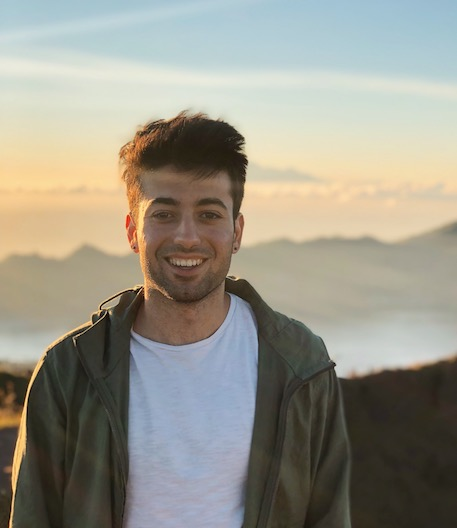
\includegraphics[width=0.2\linewidth]{assets/arda.jpg}
		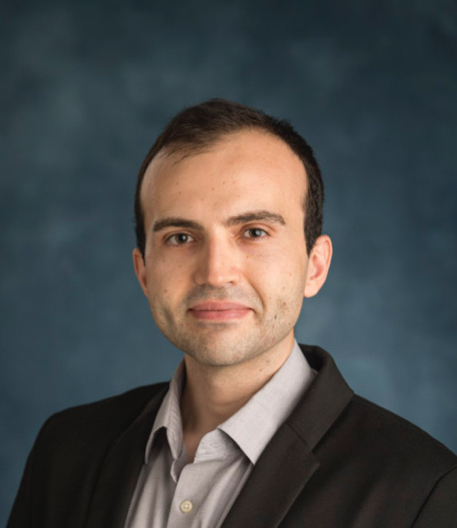
\includegraphics[width=0.2\linewidth]{assets/mert.jpg}
    }

\titlegraphic{
\includegraphics[width=0.4\textwidth]{assets/SUSig_2color_Stree_Left.eps}}

%\logo{
\includegraphics[height=0.5cm]{assets/Block_S_2_color.eps}}

%\institute{Stanford University}
\date{}

\begin{document}

\maketitle
%% main content starts %%

\begin{frame}{Motivation: Neural Networks}

	Neural networks are building blocks for modern learning systems.
	\vspace{0.5em}
	\begin{itemize}
		\item \textbf{Vision}: object recognition, localization, and bounding.
		\item \textbf{Language}: audio transcription and machine translation.
		\item \textbf{Control}: robotics, autonomous cars, game-playing, \ldots
	\end{itemize}

	\vspace{0.5em}

	\begin{columns}
		\begin{column}{0.6\textwidth}
			\centering
			\textit{A bowl of soup that is a portal to another
				dimension as digital art.}
		\end{column}
		\begin{column}{0.45\textwidth}
			\begin{figure}[]
				\centering
				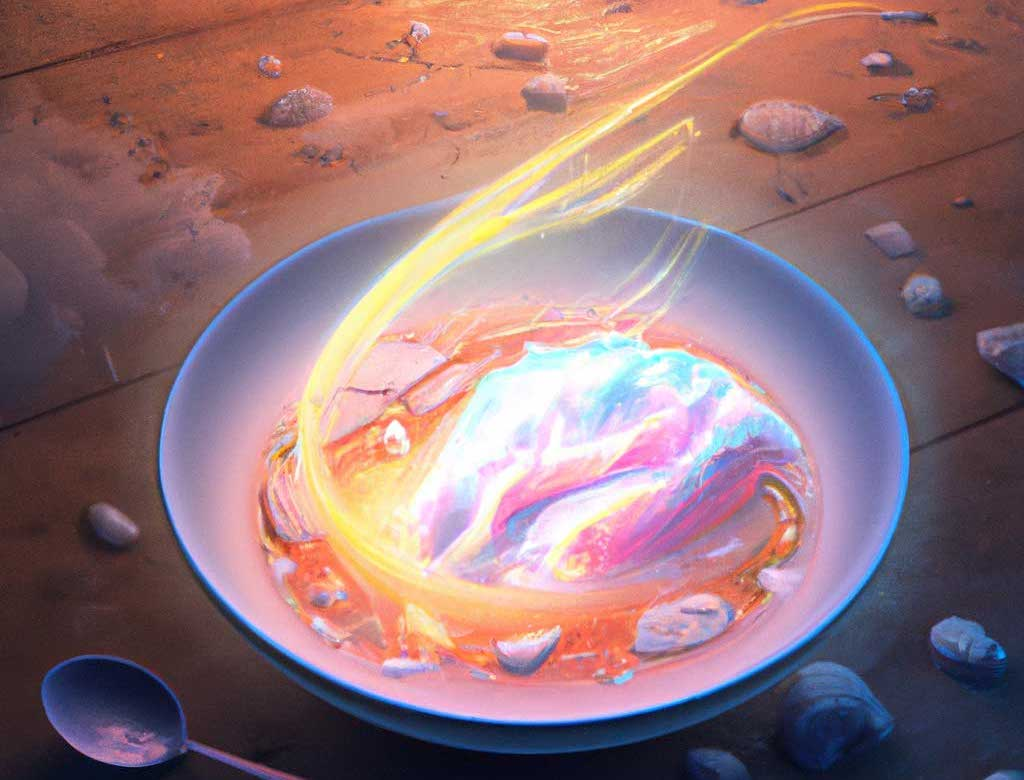
\includegraphics[width=0.8\linewidth]{assets/bowl_of_soup.jpg}
				\caption*{Generated by DALL$\cdot$E 2}%
			\end{figure}
		\end{column}
	\end{columns}

	\vspace{0.5em}

	\begin{center}
		\Large
		But optimizing neural networks is \textcolor{red}{hard}!
	\end{center}

	\source{https://openai.com/dall-e-2/}

\end{frame}

\begin{frame}{Motivation: Non-Convex Optimization}

	\begin{center}
		\Large
		DALL$\cdot$E 2 has 5.5 billion parameters and took billions of iterations to fit \citep{ramesh2022dalle}.
	\end{center}

	\vspace{1em}

	Neural network optimization is \textcolor{red}{non-convex}!
	\vspace{0.2em}
	\begin{itemize}
		\item \textbf{NP-Hard}: many sub-optimal local minima, saddles.
		\item \textbf{Speed/Stability}: tuning is critical for performance.
		\item \textbf{Model Churn}: hyper-parameters affect the final model~\citep{henderson2018deep}.
	\end{itemize}

	\begin{figure}[b]
		\centering
		%! TEX root = ../../main.tex
%% Illustration of step-sizes bound from Armijo line-search. 

\begin{tikzpicture}[scale=0.9,
		declare function={
				objective(\x)=      (\x<=-1) * (2*\x*\x + 6*\x + 4)    +
				and(\x>-1, \x<=1) * (\x + 5 - pow(\x,3) - 5*\x*\x) / 4 +
				(\x>1) * (\x*\x - 5*\x + 4);
			}
	]
	\begin{axis}[
			width=0.9\textwidth,
			height=4cm,
			axis x line=none, axis y line=none,
			ymin=-3.25, ymax=5, ytick={-5,...,5}, ylabel=$y$,
			xmin=-5, xmax=7, xtick={-5,...,7}, xlabel=$x$,
		]

		\addplot[name path=function, domain=-3.5:5.23, samples=100, line width=2pt]{objective(x)};

        \node[label={[text=blue]90:$x^*$},circle,fill=blue,inner sep=2pt] at (axis cs:2.5,-2.25) {};
        \node[label={[text=red]90:$\tilde x$},circle,fill=red,inner sep=2pt] at (axis cs:0.09717,1.3) {};
        \node[label={[text=red]90:$\tilde x$},circle,fill=red,inner sep=2pt] at (axis cs:-1.5,-0.5) {};

		\node[label={0:$f(x)$}] at (axis cs:4.2,0.8) {};
	\end{axis}
\end{tikzpicture}


	\end{figure}

\end{frame}

\begin{frame}{Convex Reformulations}

	\vspace{0.2em}
	{\large \textcolor{Red}{Non-Convex Problem}}
	\vspace{-1em}
	\begin{columns}
		\centering
		\begin{column}{0.2\linewidth}
			\small
			\[
				\begin{aligned}
					\min_{w, \alpha} & \norm{\sum_{j=1}^m (X w_j)_+ \alpha_j - y}_2^2             \\
					                 & \quad + \lambda \sum_{j=1}^m \norm{w_j}_2^2 + |\alpha_j|^2
				\end{aligned}
			\]
		\end{column}

		\begin{column}{0.7\linewidth}
			\begin{figure}[t]
				\raggedleft
				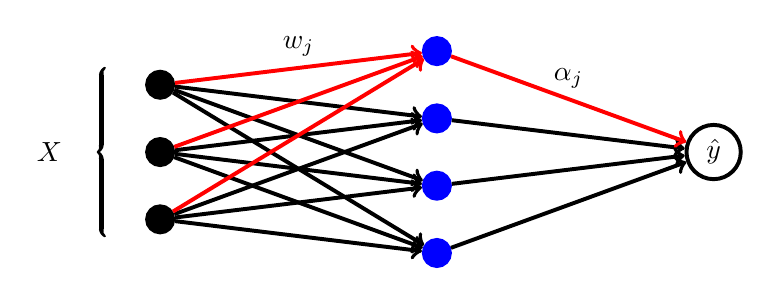
\begin{tikzpicture}[scale=1,
	]
	\begin{axis}[width=\linewidth, height=5cm,
			axis lines=none,  % don't print axis lines
			yticklabels={,,}, xticklabels={,,},
			ymin=0, ymax=8, y axis line style={-},
			xmin=0, xmax=15, x axis line style={-},
		]
		\node [] (input) at (axis cs:1,4) {$X$};
		\node [Input] (input1) at (axis cs:3,2) {};
		\node [Input] (input2) at (axis cs:3,4) {};
		\node [Input] (input3) at (axis cs:3,6) {};

		\draw [decorate, line width = 0.6mm,
			decoration = {calligraphic brace}] (axis cs:2,1.5) --  (axis cs:2,6.5);

		\node [Hidden] (hidden1) at (axis cs:8,1) {};
		\node [Hidden] (hidden2) at (axis cs:8,3) {};
		\node [Hidden] (hidden3) at (axis cs:8,5) {};
		\node [Hidden] (hidden4) at (axis cs:8,7) {};

		\draw [->, style=arrow, draw=black] (input1) -- (hidden1);
		\draw [->, style=arrow, draw=black] (input2) -- (hidden1);
		\draw [->, style=arrow, draw=black] (input3) -- (hidden1);

		\draw [->, style=arrow, draw=black] (input1) -- (hidden2);
		\draw [->, style=arrow, draw=black] (input2) -- (hidden2);
		\draw [->, style=arrow, draw=black] (input3) -- (hidden2);

		\draw [->, style=arrow, draw=black] (input1) -- (hidden3);
		\draw [->, style=arrow, draw=black] (input2) -- (hidden3);
		\draw [->, style=arrow, draw=black] (input3) -- (hidden3);

		\draw [->, style=arrow, draw=red] (input1) -- (hidden4);
		\draw [->, style=arrow, draw=red] (input2) -- (hidden4);
		\draw [->, style=arrow, draw=red] (input3) -- (hidden4) node[pos=0.5,above] {$w_j$};

		\node [Output] (output) at (axis cs:13,4) {$\hat y$};

		\draw [->, style=arrow, draw=black] (hidden1) -- (output);
		\draw [->, style=arrow, draw=black] (hidden2) -- (output);
		\draw [->, style=arrow, draw=black] (hidden3) -- (output);
		\draw [->, style=arrow, draw=red] (hidden4) -- (output) node[pos=0.5,above] {$\alpha_j$};
	\end{axis}

\end{tikzpicture}%

%\begin{tikzpicture}[scale=1,
%    ]
%    \begin{axis}[width=1.1\linewidth, height=5cm,
%            axis lines=none,  % don't print axis lines
%            yticklabels={,,}, xticklabels={,,},
%            ymin=-0.2, ymax=10.2, x axis line style={-},
%            xmin=-0.2, xmax=20.2, y axis line style={-},
%        ]

%        \filldraw[color=blue!60, fill=blue!5, line width=0.4mm](axis cs:0,5.8) rectangle (axis cs:20, 10);
%        \filldraw[color=red!60, fill=red!5, line width=0.4mm](axis cs:0,0) rectangle (axis cs:20, 4.2);

%        % non-convex models
%        \filldraw[line width=0.4mm, fill=white](axis cs:1,1) rectangle (axis cs:8, 3.2) node[pos=.5] {NC-GReLU};
%        \filldraw[line width=0.4mm, fill=white](axis cs:12,1) rectangle (axis cs:19, 3.2) node[pos=.5] {NC-ReLU};

%        % convex models
%        \filldraw[line width=0.4mm, fill=white](axis cs:1,6.8) rectangle (axis cs:8, 9) node[pos=.5] {C-GReLU};
%        \filldraw[line width=0.4mm, fill=white](axis cs:12,6.8) rectangle (axis cs:19, 9) node[pos=.5] {C-ReLU};

%        \draw [<->, solid, draw=black, line width = 0.6mm] (axis cs:4.5,3.2) -- (axis cs:4.5,6.8) node[right, pos=0.5] {\small Sol. Map};

%        \draw [<->, solid, draw=black, line width = 0.6mm] (axis cs:15.5,3.2) -- (axis cs:15.5,6.8)  node[right, pos=0.5] {\small Sol. Map};

%        \draw [<-, solid, draw=black, line width = 0.6mm] (axis cs:6,9) -- [bend left=15] (axis cs:14, 9);

%        \draw [->, solid, draw=orange, line width = 0.6mm] (axis cs:8,7.9) -- (axis cs:12,7.9);
%        \node[align=center] at (axis cs:10.1, 7.8) {\small Cone\\ \small Decomp.};
%    \end{axis}

%\end{tikzpicture}%


			\end{figure}
		\end{column}
	\end{columns}


	\pause

	{
		\vspace{-0.5em}
		\center \rule{\textwidth}{0.1em}
		\vspace{-0.2em}
	}

	{\large \textcolor{ForestGreen}{Convex Reformulation}}
	\vspace{-2em}
	\begin{columns}
		\begin{column}{0.2\linewidth}
			\vspace{1.5em}
			\small
			\[
				\begin{aligned}
					\min_{u} & \norm{\sum_{j=1}^p D_j X u_j - y}_2^2 +
					\lambda \sum_{j=1}^p \norm{u_j}_2,                 \\
					         & \hspace{0.2em} \text{where }
					D_j = \text{diag}[\mathbbm{1}(X g_i \geq 0)]
				\end{aligned}
			\]
		\end{column}
		\begin{column}{0.7\linewidth}
			\vspace{-1.5em}
			\begin{figure}[t]
				\raggedleft
				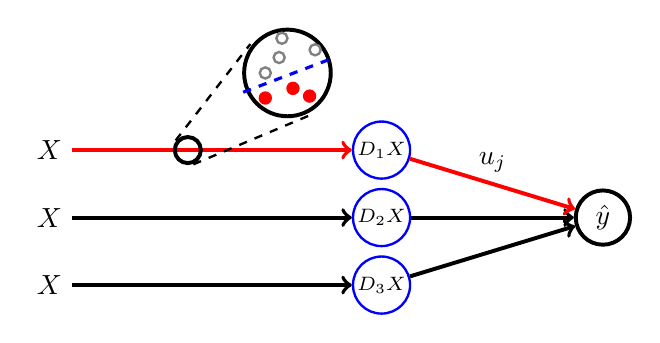
\begin{tikzpicture}[scale=1,
	]
	\begin{axis}[width=\linewidth, height=5.5cm,
			axis lines=none,  % don't print axis lines
			yticklabels={,,}, xticklabels={,,},
			ymin=0, ymax=8, y axis line style={-},
			xmin=0, xmax=15, x axis line style={-},
		]
		\node [] (input1) at (axis cs:3,1) {$X$};
		\node [] (input2) at (axis cs:3,2.75) {$X$};
		\node [] (input3) at (axis cs:3,4.5) {$X$};

        \node [Splits] (hidden1) at (axis cs:9,1) {\scriptsize $D_3 X$};
		\node [Splits] (hidden2) at (axis cs:9,2.75) {\scriptsize $D_2 X$};
		\node [Splits] (hidden3) at (axis cs:9,4.5) {\scriptsize $D_1 X$};

		\draw [->, style=arrow, draw=black] (input1) -- (hidden1);

		\draw [->, style=arrow, draw=black] (input2) -- (hidden2);

		\draw [->, style=arrow, draw=red] (input3) -- (hidden3);

		\node [Output] (output) at (axis cs:13,2.75) {$\hat y$};

		\draw [->, style=arrow, draw=black] (hidden1) -- (output);
		\draw [->, style=arrow, draw=black] (hidden2) -- (output);
		\draw [->, style=arrow, draw=red] (hidden3) -- (output) node[pos=0.5,above] {$u_j$};

		\draw [draw=black, line width=0.3mm, dashed] (axis cs:5.6, 4.13) -- (axis cs:7.7,5.4);
		\draw [draw=black, line width=0.3mm, dashed] (axis cs:5.28, 4.75) -- (axis cs:6.63,7.25);

		\node [draw=black, minimum size=0.3cm, shape=circle, solid, line width=0.5mm] (examine) at (axis cs:5.5,4.5) {};
		\node [draw=black, minimum size=1.1cm, shape=circle, solid, line width=0.5mm] (closeup) at (axis cs:7.3,6.5) {};

		\node [fill=white, draw=gray, line width=0.3mm, inner sep=0.05cm, shape=circle] at (axis cs:7.8,7.1) {};
		\node [fill=white, draw=gray, line width=0.3mm, inner sep=0.05cm, shape=circle] at (axis cs:7.15,6.9) {};
		\node [fill=white, draw=gray, line width=0.3mm, inner sep=0.05cm, shape=circle] at (axis cs:7.2,7.4) {};
		\node [fill=white, draw=gray, line width=0.3mm, inner sep=0.05cm, shape=circle] at (axis cs:6.9,6.5) {};

		\draw [draw=Blue, dashed, line width=0.4mm] (axis cs:6.5,6.) -- (axis cs:8.15,6.9);

		\node [fill=Red, inner sep=0.06cm, shape=circle] at (axis cs:6.9,5.85) {};
		\node [fill=Red, inner sep=0.06cm, shape=circle] at (axis cs:7.4,6.1) {};
		\node [fill=Red, inner sep=0.06cm, shape=circle] at (axis cs:7.7,5.9) {};

	\end{axis}

\end{tikzpicture}%

%\begin{tikzpicture}[scale=1,
%    ]
%    \begin{axis}[width=1.1\linewidth, height=5cm,
%            axis lines=none,  % don't print axis lines
%            yticklabels={,,}, xticklabels={,,},
%            ymin=-0.2, ymax=10.2, x axis line style={-},
%            xmin=-0.2, xmax=20.2, y axis line style={-},
%        ]

%        \filldraw[color=blue!60, fill=blue!5, line width=0.4mm](axis cs:0,5.8) rectangle (axis cs:20, 10);
%        \filldraw[color=red!60, fill=red!5, line width=0.4mm](axis cs:0,0) rectangle (axis cs:20, 4.2);

%        % non-convex models
%        \filldraw[line width=0.4mm, fill=white](axis cs:1,1) rectangle (axis cs:8, 3.2) node[pos=.5] {NC-GReLU};
%        \filldraw[line width=0.4mm, fill=white](axis cs:12,1) rectangle (axis cs:19, 3.2) node[pos=.5] {NC-ReLU};

%        % convex models
%        \filldraw[line width=0.4mm, fill=white](axis cs:1,6.8) rectangle (axis cs:8, 9) node[pos=.5] {C-GReLU};
%        \filldraw[line width=0.4mm, fill=white](axis cs:12,6.8) rectangle (axis cs:19, 9) node[pos=.5] {C-ReLU};

%        \draw [<->, solid, draw=black, line width = 0.6mm] (axis cs:4.5,3.2) -- (axis cs:4.5,6.8) node[right, pos=0.5] {\small Sol. Map};

%        \draw [<->, solid, draw=black, line width = 0.6mm] (axis cs:15.5,3.2) -- (axis cs:15.5,6.8)  node[right, pos=0.5] {\small Sol. Map};

%        \draw [<-, solid, draw=black, line width = 0.6mm] (axis cs:6,9) -- [bend left=15] (axis cs:14, 9);

%        \draw [->, solid, draw=orange, line width = 0.6mm] (axis cs:8,7.9) -- (axis cs:12,7.9);
%        \node[align=center] at (axis cs:10.1, 7.8) {\small Cone\\ \small Decomp.};
%    \end{axis}

%\end{tikzpicture}%


			\end{figure}
		\end{column}
	\end{columns}
\end{frame}

\begin{frame}{Convex Reformulations: A Huge-Scale Linear Model}
	\vspace{-2em}
	\[
		\begin{aligned}
			\textbf{Convex Form}: \quad
			\min_{u} \; & \norm{\sum_{j=1}^p D_j X u_j - y}_2^2 +
			\lambda \sum_{j=1}^p \norm{u_j}_2,                    \\
			            & \hspace{0.2em} \text{where }
			D_j = \text{diag}[\mathbbm{1}(X g_i \geq 0)]
		\end{aligned}
	\]
	\begin{itemize}
		\item \textcolor{red}{Exponential in general}: \( p \in O(r \cdot (\frac{n}{r})^r) \),
		      where \( r = \text{rank}(X) \).
		      \vspace{0.2em}

		\item But, \( D_j X \) is \textcolor{ForestGreen}{row-sparse}, \( u \) is \textcolor{ForestGreen}{sparse} when
		      \( \lambda \gg 0 \), and the objective is \textcolor{ForestGreen}{quadratic} + simple non-smooth.
	\end{itemize}

	\pause

	{
		\vspace{-0.5em}
		\center \rule{\textwidth}{0.1em}
		\vspace{-0.2em}
	}
	Solve with (accelerated) \textbf{proximal-gradient} methods:
	\begin{align*}
		u_i^+
		 & = u_i^k - \etak X^\top D_i^\top \rbr{\sum_{j=1}^p D_j X u_j - y} \\
		u_i^{k+1}
		 & = u_i^+ \rbr{1 - \frac{\etak \cdot \lambda}{\norm{u_i^+}_2}}_+
	\end{align*}

\end{frame}

\begin{frame}{Convex Reformulations: Performance}

	Fast solvers use \textbf{numerical tricks} and \textbf{hardware acceleration}:
	\vspace{1em}
	\begin{itemize}
		\item \textcolor{ForestGreen}{Classic Tricks}: faster convergence via line-search, restarts, \ldots
		\item \textcolor{ForestGreen}{CUDA GPUs}: \( 70\times \) faster Mat-Vec operations using \texttt{float32}.
		\item \textcolor{ForestGreen}{Code Optimization}: tensor operations remove intermediate computations,
		      data normalization improves conditioning, \ldots
	\end{itemize}
	\vspace{1em}

	\textcolor{red}{Scaling} is a still a problem!
	\begin{itemize}
		\item Dense operations on GPUs are faster than sparse computations with OpenMP --- does this reverse at scale?
		\item GPU memory is typically 32GB, but ImageNet is 150GB --- can we use multi-GPU programming models?
		\item How can we leverage the (dynamic) sparsity pattern of \( u^k \)?
	\end{itemize}

\end{frame}

%% main content ends %%

%% end slide
\setbeamercolor{background canvas}{bg=LightCyan}

\begin{frame}{}
	\begin{center}
		\huge Thanks for Listening!
	\end{center}
\end{frame}
\setbeamercolor{background canvas}{bg=white}

%% bibliography
\begin{frame}[allowframebreaks]{References}
	\printbibliography[]
\end{frame}


\end{document}
